\begin{exo}
  \donnee{Considérons deux variables aléatoires X et Y dont les histogrammes se trouvent dans la figure ci-dessous.\\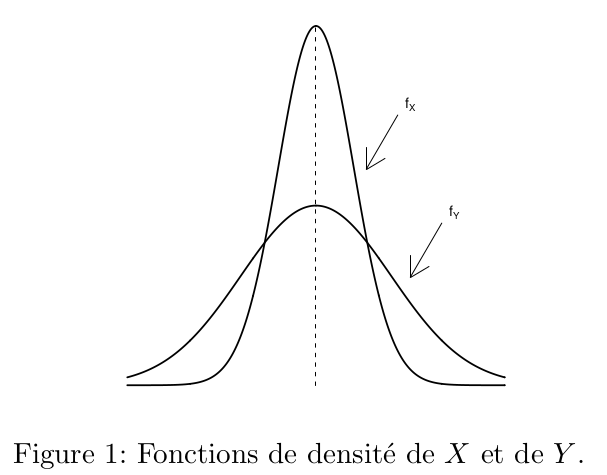
\includegraphics[width=8cm]{ex5.png}
  \\En n’effectuant aucun calcul, l’écart-type de X est-il plus grand que celui de Y ?
  }
  L'écart type est plus grand dans la figure x car les données sont plus écartées que dans la figure y
\end{exo}
